\usetikzlibrary{positioning}

\begin{document}

\def\title{Worksheet 5}

\newcommand{\qitem}{\qpart\item}

\renewcommand{\labelenumi}{(\alph{enumi})} % change default enum format to (a)
\renewcommand{\theenumi}{(\alph{enumi})} % fix reference format accordingly.
\renewcommand{\labelenumii}{\roman{enumii}.} % second level labels.
\renewcommand{\theenumii}{\roman{enumii}.}

\maketitle

\vspace{0.5em}

\begin{qunlist}
% {\Large \textbf{Mechanical:}}
\qns{Change of Coordinates}
\qcontributor{Yi Zhao, Son Tran, Naomi Sagan, Taejin Hwang}

Many engineering problems can be difficult to solve in its standard xyz coordinates, but may be much easier in a different coordinate system.
In this problem, we will review the process of \emph{change of basis} between coordinate systems.
Remember that a \emph{change of basis} can be represented by a invertible, square matrix.
\par

Let's first start with an example.
Consider the vector $\vec{u} = [u_1, u_2]^T.$ When we write a vector in this form, implicitly we are representing it with the \emph{standard basis} for $\R^{2}$, $\vec{e_1} = [1, 0]^T$ and $\vec{e_2} = [0, 1]^T.$ 

This means that we can write $\vec{u}$ as a linear combination using standard basis vectors $\vec{u} = u_1\vec{e_1} + u_2\vec{e_2}$.
\par

Now, what if we want to represent $\vec{u}$ as a linear combination of another set of basis vectors, say $\vec{a_1} = [1, 1]^T$ and $\vec{a_2} = [0, -1]^T?$
This means that we need to find scalars $u_{a_1}$ and $u_{a_2}$ such that $\vec{u} = u_{a_1}\vec{a_1} + u_{a_2}\vec{a_2}$.
We can write this equation in matrix form:
\[
  \begin{bmatrix}
    | & | \\
    \vec{a_1} & \vec{a_2} \\
    | & |
  \end{bmatrix}
  \begin{bmatrix} u_{a_1} \\ u_{a_2} \end{bmatrix} = \begin{bmatrix} u_{1} \\ u_{2} \end{bmatrix}
.\]
Thus we can find $u_{a_1}$ and $u_{a_2}$ by solving a system of linear equations as seen in 16A.
\par

\meta{
  You can also explain to students that there must be a unique solution, since the U matrix is invertible.
}


\begin{enumerate}
  % Part(a)
  \qitem Let $\vec{v} = [2,-1]^{T}$. What equation gives the coordinates of $\vec{v}$ in the below basis? 
  Try to express your answer in matrix-vector form. No need to do the full calculation.

  \begin{gather*}
    \vec{x} =
    \begin{bmatrix}
      4 \\
      -2
    \end{bmatrix},
    \vec{y} = \begin{bmatrix}
      -3 \\
      -3
    \end{bmatrix}
  \end{gather*}

  % Part(a) solution
  \sol{

    In general, suppose we are given a vector $\vec{u} \in \R^{n}$ in the standard basis and want to change to a different basis with basis vectors $\vec{a_1}, \cdots, \vec{a_n}$.
    If we denote the vector in the new basis as $\vec{u_a} = \begin{bmatrix} u_{a_1} \\ \vdots \\ u_{a_n} \end{bmatrix}$, we solve the following equation $A\vec{u_a} = \vec{u}$, where A is the matrix $\begin{bmatrix} \vec{a_1} & \cdots & \vec{a_n} \end{bmatrix}$.
    Therefore the change of basis is given by:
    \[
      \vec{u_a} = A^{-1}\vec{u}
    .\]

    $$
    \vec{u_a} =
    \begin{bmatrix}
      4 & -3 \\
      -2 & -3
    \end{bmatrix}^{-1}
    \begin{bmatrix}
      2 \\
      -1
    \end{bmatrix}
    $$
  }

  % Part(b)
  \qitem Let $\vec{v} = [3,3]^{T}$. We are told that $\vec{v}$ is represented in the basis:

  \begin{gather*}
    \vec{x} =
    \begin{bmatrix}
      1 \\
      1
    \end{bmatrix},
    \vec{y} = \begin{bmatrix}
      1 \\
      -1
    \end{bmatrix}
  \end{gather*}
  What equation gives the coordinates of $\vec{v}$ in the standard basis?

  % Part(b) solution
  \sol {
    If we already have a vector $\vec{u_a}$ in the basis $\vec{a_1}, \cdots, \vec{a_n}$, how do we change it back to a vector $\vec{u}$ in the standard basis?
    We can reverse the change of basis transformation, thus $\vec{u} = A\vec{u_a}$.
    \par

    $$
    \vec{u_a} =
    \begin{bmatrix}
      1 & 1 \\
      1 & -1
    \end{bmatrix}
    \begin{bmatrix}
      3 \\
      3
    \end{bmatrix}
    $$
  }

 \end{enumerate}

 Now that we've had some mechanical practice, we'll look more into the input-output relationship of vectors.
 For the remaining parts, we'll refer to $[\vec{x}]_S$ or $\vec{x}$ as a vector using standard basis coordinates, and $[\vec{x}]_\beta$ as a vector using $\beta$ basis coordinates.

% Part(c)
 \begin{enumerate}[resume]
  \qitem Let $[\vec{x}]_\beta$ be a vector in $\beta$ coordinates, and $V$ be a change of coordinates matrix from $S \to \beta.$ \\
  How can we represent $\vec{x}$ in terms of $[\vec{x}]_\beta$ and $V?$

  \sol {
    We are given a matrix $V$ that converts standard coordinates to $\beta$ coordinates. 
    This means that $V^{-1}$ will be a matrix that converts $\beta$ coordinates to standard coordinates.
    Therefore, in order to get $\vec{x},$ we multiply $V^{-1}$ with $[\vec{x}]_\beta:$
    $V^{-1} \cdot [\vec{x}]_\beta = [\vec{x}]_S = \vec{x}.$
  }

  % Part(d)
  \qitem Now let $B$ be a linear operator in $\beta$ coordinates. This means that it will take in a vector $[\vec{x}]_\beta$ as an input and output $[\vec{y}]_\beta.$ Given a vector $\vec{x}$ in standard coordinates, why can't we multiply $B \vec{x}$ to get the output $\vec{y}$ in standard coordinates?

  \sol{
    The transformation $B$ "lives" in a different world. It can only accept vectors in $\beta$ coordinates as inputs. 
    Therefore, in order to solve this, we must convert $\vec{x}$ into $\beta$ coordinates.
  }

  % Part(e)
  \qitem Using our $V$ matrix given above, as the change of coordinates matrix from $S \to \beta,$ how can we describe the linear operator $B$ in standard coordinates, that is if $\vec{y} = A \vec{x},$ what is $A$ in the standard basis?

  \sol {
    There will be two main issues we need to address in this question. First off, we need a $\beta$ coordinate input. Secondly, the output of the $B$ is in $\beta$ coordinates, and we will need to convert that back to standard coordinates. 

    Therefore, we take the following steps.

    1. Let's first make our input into $B$ in $\beta$ coordinates. 
    $$\text{Let } \vec{v} = V \vec{x}.$$
    2. Now if we input $\vec{v}$ we will get some output:
    $$\vec{w} = B \vec{v}.$$
    3. However, $\vec{w}$ is in $\beta$ coordinates, so we must convert back to standard coordinates using $V^{-1}.$
    $$\vec{y} = V^{-1} \vec{w}$$
    4. Cascading all of our matrix multiplications, we end up with:
    $$\vec{y} = V^{-1} B V \vec{x}.$$
    Therefore, we can see that $A = V^{-1} B V.$

    The following can also be represented in this state diagram: 

    Note that when cascading transformations, we apply them to the \textbf{left} of the existing transformation.

    \begin{figure}[H]
      \centering
      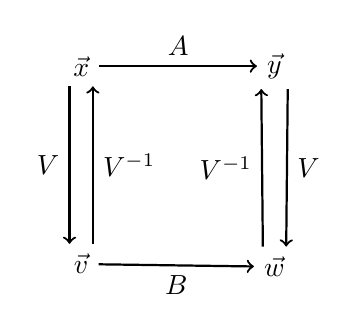
\begin{tikzpicture}[node distance = 2cm, thick]%
        \node (1) {$\vec{x}$};
        \node (2) [right=of 1] {$\vec{y}$};
        \node (3) [below=of 2] {$\vec{w}$};
        \node (4) [below=of 1] {$\vec{v}$};
        \draw[->] (1) -- node [midway,above] {$A$} (2);
        \draw[->] (1.240) -- node [midway,left]{$V$} (4.120);
        \draw[->] (4.60) -- node [midway,right]{$V^{-1}$} (1.300);
        \draw[->] (2.300) -- node [midway,right]{$V$} (3.60);
        \draw[->] (3.120) -- node [midway,left]{$V^{-1}$} (2.240);
        \draw[->] (4) -- node [midway,below] {$B$} (3);
      \end{tikzpicture}%
    \end{figure}
  }
  % % Part(c) solution
  % \sol{
  %   Start by writing $\vec{x_1}$ in terms of $\vec{z_1}$:
  %   $$ \vec{x_1} = V \vec{z_1} $$
  %   Then, apply the transformation $A$ to $\vec{x_1}$, substituting $V \vec{z_1}$ for $\vec{x_1}$:
  %   $$ \vec{x_2} = A V \vec{x_1} $$
  %   Finally, left-multiply both sides by $V^{-1}$ to change $\vec{x_2}$ to the eigenbasis:
  %   $$ \vec{z_2} = V^{-1} \vec{x_2} = V^{-1} A V \vec{z_1} $$

  %   $$A' = V^{-1} A V =
  %   \begin{bmatrix}
  %     1 & 1 \\
  %     -2 & 1
  %   \end{bmatrix}^{-1}
  %   \begin{bmatrix}
  %     3 & -1 \\
  %     -2 & 4
  %   \end{bmatrix}
  %   \begin{bmatrix}
  %     1 & 1 \\
  %     -2 & 1
  %   \end{bmatrix}
  %   $$

  %   $A'$ represents the transformation $A$ in the eigenbasis of $A$, so we know that $A'$ is the diagonal matrix:
  %   $$ A' =
  %   \begin{bmatrix}
  %     \lambda_1 & 0 \\
  %     0 & \lambda_2
  %   \end{bmatrix} =
  %   \begin{bmatrix}
  %     5 & 0 \\
  %     0 & 2
  %   \end{bmatrix} $$

  %   In general, suppose we have a linear transformation $T$ represented by a $n \times n$ matrix that transforms $\vec{u} \in \R^{n}$ to $\vec{v} \in \R^{n}$:
  %   \[
  %     \vec{v} = T\vec{u}
  %   .\]
  %   Suppose we have a basis vectors $\vec{a_1}, \cdots, \vec{a_n} \in \R^{n}$, and the vectors $\vec{u}, \vec{v}$ above are represented in this basis:
  %   \[
  %     \begin{aligned}
  %       \vec{u_a} &= u_{a_1}\vec{a_1} + \cdots + u_{a_n}\vec{a_n} \\
  %       \vec{v_a} &= v_{a_1}\vec{a_1} + \cdots + v_{a_n}\vec{a_n}.
  %     \end{aligned}
  %   \]
  %   Thus we have
  %   \[
  %     \begin{aligned}
  %       T\vec{u}          &= \vec{v} \\
  %       TA\vec{u_a}       &= A\vec{v_a} \\
  %       A^{-1}TA\vec{u_a} &= \vec{v_a}.
  %     \end{aligned}
  %   \]
  %   By pattern matching, we see that if we set $T_a = A^{-1}TA$, we get the relationship $T_a\vec{u_a} = \vec{v_a}$ in the new basis.
  %   The correspondences stated above are all represented in the following diagram:
  %   % \begin{figure}[H]
  %   %   \centering
  %   %   \includegraphics[scale=0.1]{\bank/statespace/figures/change_of_basis.jpg}
  %   % \end{figure}
\end{enumerate}

\newpage
% Authors: Tony Li, and authors of diagonalization.tex
% Email: songli@berkeley.edu

\qns{Diagonalization and Diagonalizability}

\textbf{Diagonal matrices}, matrices where all entries outside of the diagonal are zero.
Diagonal matrices come handy in terms of solving systems of linear equations, solving for vector case of differential equations, finding out the determinant, etc. 
\newline \textbf{Diagonalization} is a procedure that we transform a matrix $A$ into three matrices multiplied together, whihc means 
$A=V{\Lambda}V^{-1}$, where $V^{-1}$ is the inverse of $V$, and $\Lambda$ is a diagonal matrix.

In this problem, we'll investigate what $V$ and $\Lambda$ truly are.

\begin{enumerate}

\qitem First we need to recall some pretty useful concepts, eigenvalues and eigenvectors. For a matrix $A$, if we can write the
equation that $A\vec{v}=\lambda\vec{v}$, where $\lambda$ is non-zero and $\vec{v}$ is non-zero vector, then we say that $\vec{v}$ and $\lambda$ is a pair of eigenvector and eigenvalue of $A$.
Given that 
$$A = \begin{bmatrix}
  2 & 2 \\
  5 & -1
  \end{bmatrix}$$
\textbf{Can you explain why $A$ has two eigenvalues and in a more general case, how many eigenvalues does a n by n matrix have?}
\ws{
\vspace{30px}
}

\meta{
  Introduce how we solve for eigenvalues and eigenvectors.
}

\sol{
  Based on the definition, we know $A\vec{v}=\lambda\vec{v}$, then we can write it into another form, $(A-{\lambda}I_n)\vec{v}=0$, where $I_n$
  is the identity matrix. As a result, since $\vec{v}$ can not be a zero vector, $(A-{\lambda}I_n)\vec{v}=0$ is a homogenous linear system solving for $\vec{v}$.
  $\vec{v}$ has non zero solution, only when $A-{\lambda}I_n$ is not invertible, which implies that $det(A-{\lambda}I_n)=0$.
  Solving a $det(A-{\lambda}I_n)=0$ is essentially solving a polynomial with degree n, so \textbf{$\lambda$ should have n solutions}.
  Plase note that, $\lambda$'s could be complex numbers.
}

\qitem \textbf{Find eigenvalues ${\lambda}_1$ and ${\lambda}_2$ and their corresponding eigenvectors $\vec{v_1}$ and $\vec{v_2}$}, where ${\lambda}_1\le{\lambda}_2$,
and both of the eigenvectors have length 1.

\ws{
\vspace{100px}
}

\sol{
  $$det(A-{\lambda}I_n)=det(\begin{bmatrix}
    2-\lambda & 2\\
    5 & -1-\lambda
  \end{bmatrix})=(2-\lambda)(-1-\lambda)-2\times5={\lambda}^2-\lambda-12=0$$
  \newline After solving the quadratic equation above, We have ${\lambda}_1=-3$ and ${\lambda}_2=4$.
  Let's plug two eigenvalues into $(A-{\lambda}I_n)\vec{v}=0$.
  $$\begin{bmatrix}
    2-{\lambda}_1 & 2\\
    5 & -1-{\lambda}_1 
  \end{bmatrix}\vec{v_1} = \begin{bmatrix}
    5 & 2\\
    5 & 2
  \end{bmatrix}\vec{v_1}=0$$
  $$\Rightarrow \vec{v_1}=\begin{bmatrix}
    2C\\
    -5C\\
  \end{bmatrix}, C\in\mathbb{R}$$
  Since $\vec{v_1}$ has length 1, then $$\vec{v_1}=\begin{bmatrix}
    \frac{2}{\sqrt{29}}\\
    \frac{-5}{\sqrt{29}}
  \end{bmatrix}$$
  \newline Similarly, we would have 
  $$\vec{v_2}=\begin{bmatrix}
    \frac{1}{\sqrt{2}}\\
    \frac{1}{\sqrt{2}}
  \end{bmatrix}$$
}

\end{enumerate}

With the eigenvectors $\vec{v_1}$ and $\vec{v_2}$, define $V$ to be the matrix:
$$V = \begin{bmatrix}
\vec{v_1} & \vec{v_2}
\end{bmatrix}$$
Columns of this matrix $V$ are called eigenbasis of $A$.
With the eigenvalues ${\lambda}_1$ and ${\lambda}_2$, define $\Lambda$ to be the matrix:
$$\Lambda = \begin{bmatrix}
  {\lambda}_1 & 0\\
  0 & {\lambda}_2
  \end{bmatrix}$$
\begin{enumerate}[resume]
\qitem Now, we need to \textbf{prove that $A=V{\Lambda}V^{-1}$}. Assume that $V$ is invertible.
\newline \emph{Hint:}First, transform the above equation into the form $AV=V{\Lambda}$. Then, expand $V$ and $\Lambda$ with
matrices provided above.
\ws{\vspace{100px}}

\meta{
  Show students that the procedure in the solution is applicable to prove $A=V{\Lambda}V^{-1}$, even if A is n by n.
}

\sol{
  Based on the definition of eigenvalues and eigenvectors, let $\vec{v_1}$, $\vec{v_2}$,..., $\vec{v_n}$ be n eigenvectors
  of the n by n matrix $A$, and their corresponding eigenvalues are ${\lambda}_1$, ${\lambda}_2$,..., ${\lambda}_n$.
  Now, we have $V=[\vec{v_1}, \vec{v_2}, ..., \vec{v_n}]$.
  $$AV=A[\vec{v_1}, \vec{v_2}, ..., \vec{v_n}]=[A\vec{v_1}, A\vec{v_2}, ..., A\vec{v_n}]=[{\lambda}_1\vec{v_1}, {\lambda}_2\vec{v_2}, ..., {\lambda}_n\vec{v_n}]$$
  $$=[\vec{v_1}, \vec{v_2}, ..., \vec{v_n}]\begin{bmatrix}
    {\lambda}_1&0&0&...\\
    0&{\lambda}_2&0&...\\
    ...&...&...&...\\
    0&0&...&{\lambda}_n
  \end{bmatrix}=V\Lambda$$
}
\qitem Now you know that in order to diagonalize a given matrix, we need to calculate eigenvalues and eigenvectors first. However, there is still a premise we need to deal with: \textbf{when is a matrix diagonalizable?
If a matrix is diagonalizable, does it imply that the matrix is also invertible? In the opposite direction, is an invertible matrix always diagonalizable?}
\ws{\vspace{40px}}

\meta{
  The essence of this question is to tell students that invertibility does not work here, and most students would tend to use invertibility
  to explain diagonalizability.
}

\sol {
  If we look at the steps of proving $A=V{\Lambda}V^{-1}$, we made assumption that proving $A=V{\Lambda}V^{-1}$ is equivalent to
  proving $AV=V\Lambda$. The only difference here is whether $V$, or the eigenbasis, is invertible. Therefore, if a matrix is diagonalizable,
  its eigenbasis should have n linearly independent eigenvectors, or the eigenbasis is invertible, or the determinant of eigenbasis is not 0.
  \newline The invertibility of the matrix itself does not imply its diagonalizability, and the diagonalizability also does not imply invertibility.
  \newline Counterexample of the first claim: 
  $$M=\begin{bmatrix}
    1&1\\
    0&1
  \end{bmatrix}$$
  Here, $M$ is invertible since $det(M)\ne0$, but it have two equal-value eigenvalues 1, which means that two eigenvectors can not be not
  linearly independent, so it is not diagonalizable.
  \newline Counterexample of the second claim:
  $$N=\begin{bmatrix}
    0&0\\
    0&1
  \end{bmatrix}$$
  In this case, $N$ is diagonalizable, since it has two distinct eigenvalues ${\lambda}_1=0$ and ${\lambda}_2=1$. Eigenvectors corresponding to distinct eigenvalues are linearly independent.
  However, $N$ is not invertible, because $det(N)=0$.
}
\end{enumerate}
Let's now concentrate on the diagonalization with help of change of basis. We'll explore the diagonalization more clearly from the
perspective of change of basis.
\begin{enumerate}[resume]

\qitem Let $\widetilde{\vec{x}}$ be the coordinates of $\vec{x}$ in the eigenbasis. 
This means that for some arbitrary vector represented in the eigenbasis $\widetilde{\vec{x}} = \begin{bmatrix} \alpha_1 \\ \alpha_2 \end{bmatrix}$, 
the corresponding representation in standard coordinates is a linear combination of the columns of $V$: $\vec{x} = \alpha_1 \vec{v_1} + \alpha_2 \vec{v_2}$. \textbf{What is $\widetilde{\vec{x}}$ in terms of $V$ and $\vec{x}?$}

(\textit{Hint: Write $\vec{x}$ in terms of $V$ and $\tilde{\vec{x}}$, then go from there.})

\ws{\vspace{3em}}

\meta{
  The line $\alpha_1 \vec{v_1} + \alpha_2 \vec{v_2} = V \widetilde{\vec{x}}$ is not the most intuitive.
  It may require you showing on the board, why matrix vector multiplication can be seen as a linear combination of the columns.
}

\sol{
  $\vec{x} = \alpha_1 \vec{v_1} + \alpha_2 \vec{v_2} = V \widetilde{\vec{x}}.$ So it follows that $\widetilde{\vec{x}} = V^{-1} \vec{x}.$
}

\qitem It is often helpful to visualize the change of basis in a state diagram, where \textit{each arrow represents left-multiplying the variable it's coming out of by the corresponding matrix.} \textbf{Fill in the missing matrix operations in the state diagram based on your answer from the previous part.}

\ws {
  \begin{figure}[H]
    \centering
    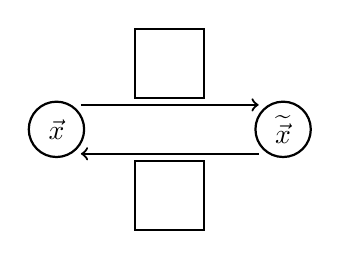
\begin{tikzpicture}[node distance = 2cm, thick,every node/.style={inner sep=0.25em,outer sep=0.25em}]%
      \node (1) [circle,draw,minimum size=2em] {$\vec{x}$};
      \node (2) [circle,draw,right=of 1,minimum size=2em] {$\widetilde{\vec{x}}$};
      \draw[->] (1.45) -- node [rectangle,draw,midway,above,minimum size=2.5em] {} (2.135);
      \draw[->] (2.225) -- node [rectangle,draw,midway,below,minimum size=2.5em] {} (1.315);
    \end{tikzpicture}%
  \end{figure}
}

\meta {
  Not everyone finds this diagram the most intuitive, but it definitely helps a large percentage of students. Stress to students that it's always better to understand the intuitive meaning behind change of basis than to remember any particular change of basis formula. This intuitive meaning is bridging between coordinate systems, which can be visualized with this diagram.
}

\sol {
  \begin{figure}[H]
  \centering
  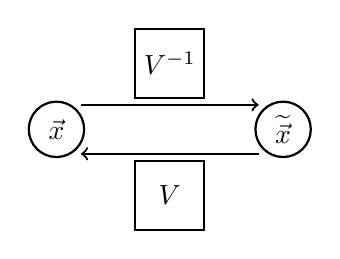
\begin{tikzpicture}[node distance = 2cm, thick,every node/.style={inner sep=0.25em,outer sep=0.25em}]%
    \node (1) [circle,draw,minimum size=2em] {$\vec{x}$};
    \node (2) [circle,draw,right=of 1,minimum size=2em] {$\widetilde{\vec{x}}$};
    \draw[->] (1.45) -- node [rectangle,draw,midway,above,minimum size=2.5em] {$V^{-1}$} (2.135);
    \draw[->] (2.225) -- node [rectangle,draw,midway,below,minimum size=2.5em] {$V$} (1.315);
  \end{tikzpicture}%
  \end{figure}
}


\qitem Now that we are able to switch back and forth between the coordinate systems, let's see how the linear transformation brought by $A$ can be viewed as a diagonal scaling transformation in the eigenbasis coordinate system.% Might be a bit confusing.

Let $\vec{y} = A \vec{x}$, and $\vec{x} = \alpha_1 \vec{v_1} + \alpha_2 \vec{v_2}$, using the same matrix $A$ and eigenvectors $\vec{v_1}, \vec{v_2}$ from before. Let $\widetilde{\vec{x}}$, $\widetilde{\vec{y}}$ be the coordinates of $\vec{x}$, $\vec{y}$ in the eigenbasis. \textbf{Find $\widetilde{\vec{x}}$ and $\widetilde{\vec{y}}$ in terms of $\alpha_1, \alpha_2, \lambda_1, \lambda_2$. What can we say about the relationship between $\widetilde{\vec{x}}$ and $\widetilde{\vec{y}}$?} % Might be confusing as to what the problem is asking compared to the next part.

(\textit{Hint}: Your answers shouldn't be in terms of the original $\vec{x}$ or $\vec{y}$.
 Use what you know about the coordinates of a vector in a certain basis; there is no need to invert any matrices or do any major computation.)

\ws {
  \vspace{200px}
}

\meta {
  Students may try to use what they found in the previous parts to multiply the vectors by $V^{-1}$. While this is technically right, make sure they understand what exactly
  that transformation is doing and why they don't need to do any matrix computation to find the coordinates of $\vec{y}$ in the eigenbasis.
}

\sol {
  $$\widetilde{\vec{x}} = \begin{bmatrix} \alpha_1 \\ \alpha_2 \end{bmatrix}$$

  \begin{align*}
    \vec{y} &= A \vec{x} \\
    &= A(\alpha_1 \vec{v_1} + \alpha_2 \vec{v_2}) \\
    &= \alpha_1 A \vec{v_1} + \alpha_2 A \vec{v_2} \\
    &= \alpha_1 \lambda_1 \vec{v_1} + \alpha_2 \lambda_2 \vec{v_2} \\
    \implies \widetilde{\vec{y}} &= \begin{bmatrix} \alpha_1 \lambda_1 \\ \alpha_2 \lambda_2 \end{bmatrix}
  \end{align*}

  This means that the matrix $D$ relating the two coordinates in the eigenbasis must be a diagonal scaling transformation, with the eigenvalues as the amount each dimension is scaled by.
}

\qitem \textbf{Find the matrix $D$ satisfying $\widetilde{\vec{y}} = D \widetilde{\vec{x}}$ in terms of $V$ and $A$.}

(\textit{Hint}: Start by writing $\vec{x}, \vec{y}$ in terms of $\widetilde{\vec{x}}$ and $\widetilde{\vec{y}}$. Refer to the state diagram from before.)

\ws{\vspace{240px}}

\meta {
  If students are comfortable with matrices representing linear transformations, you can explain this eigendecomposition as translating a linear transformation to and from the eigenbasis. For the diagonalization $A = VDV^{-1}$, left-multiplying an arbitrary vector $\vec{x}$ is equivalent to the following:

  \begin{align*}
    A \vec{x} &= VDV^{-1} \vec{x} \\
    &= VD \widetilde{\vec{x}} \\
    &= VD \begin{bmatrix} \alpha_1 \\ \alpha_2 \end{bmatrix} \\
    &= V \begin{bmatrix} \alpha_1 \lambda_1 \\ \alpha_2 \lambda_2 \end{bmatrix} \\
    &= V \widetilde{\vec{y}} \\
    &= \vec{y}
  \end{align*}
}

\sol {
  \begin{align*}
    \vec{y} &= A \vec{x} \\
    V \widetilde{\vec{y}} &= A V \widetilde{\vec{x}} \\
    \widetilde{\vec{y}} &= V^{-1} A V \widetilde{\vec{x}} \\
    \implies D &= V^{-1} A V
  \end{align*}
}

\qitem Finally, let's visualize this linear transformation $A$ from the perspective of two different coordinate systems in the state diagram below. \textbf{Fill in the missing matrix operations in the state diagram. How can you show and explain the diagonalization $A = VDV^{-1}$ (using the state diagram) and the change of basis perspective?}

\ws {
  \begin{figure}[H]
    \centering
    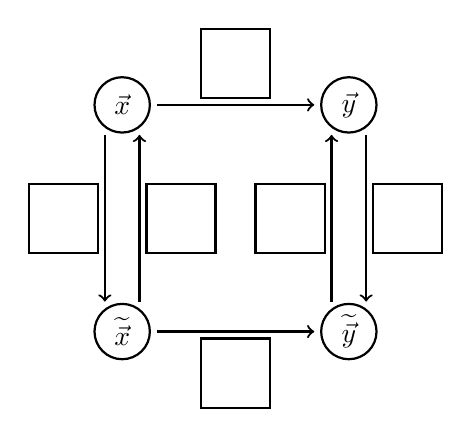
\begin{tikzpicture}[node distance = 2cm, thick, every node/.style={inner sep=0.25em,outer sep=0.25em}]%
      \node (1) [circle,draw,minimum size=2em] {$\vec{x}$};
      \node (2) [circle,draw,right=of 1,minimum size=2em] {$\vec{y}$};
      \node (3) [circle,draw,below=of 2,minimum size=2em] {$\widetilde{\vec{y}}$};
      \node (4) [circle,draw,below=of 1,minimum size=2em] {$\widetilde{\vec{x}}$};
      \draw[->] (1) -- node [rectangle,draw,midway,above,minimum size=2.5em] {} (2);
      \draw[->] (1.240) -- node [rectangle,draw,midway,left,minimum size=2.5em]{} (4.120);
      \draw[->] (4.60) -- node [rectangle,draw,midway,right,minimum size=2.5em]{} (1.300);
      \draw[->] (2.300) -- node [rectangle,draw,midway,right,minimum size=2.5em]{} (3.60);
      \draw[->] (3.120) -- node [rectangle,draw,midway,left,minimum size=2.5em]{} (2.240);
      \draw[->] (4) -- node [rectangle,draw,midway,below,minimum size=2.5em] {} (3);
    \end{tikzpicture}%
  \end{figure}
}

\sol {
  \begin{figure}[H]
    \centering
    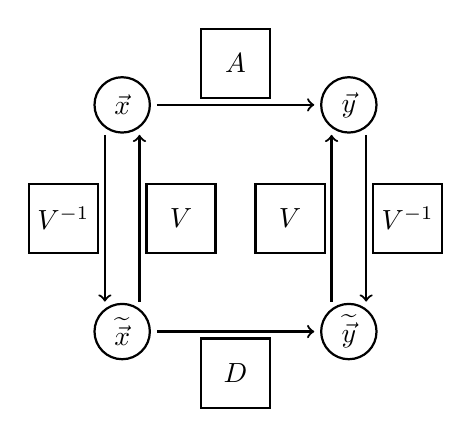
\begin{tikzpicture}[node distance = 2cm, thick, every node/.style={inner sep=0.25em,outer sep=0.25em}]%
      \node (1) [circle,draw,minimum size=2em] {$\vec{x}$};
      \node (2) [circle,draw,right=of 1,minimum size=2em] {$\vec{y}$};
      \node (3) [circle,draw,below=of 2,minimum size=2em] {$\widetilde{\vec{y}}$};
      \node (4) [circle,draw,below=of 1,minimum size=2em] {$\widetilde{\vec{x}}$};
      \draw[->] (1) -- node [rectangle,draw,midway,above,minimum size=2.5em] {$A$} (2);
      \draw[->] (1.240) -- node [rectangle,draw,midway,left,minimum size=2.5em]{$V^{-1}$} (4.120);
      \draw[->] (4.60) -- node [rectangle,draw,midway,right,minimum size=2.5em]{$V$} (1.300);
      \draw[->] (2.300) -- node [rectangle,draw,midway,right,minimum size=2.5em]{$V^{-1}$} (3.60);
      \draw[->] (3.120) -- node [rectangle,draw,midway,left,minimum size=2.5em]{$V$} (2.240);
      \draw[->] (4) -- node [rectangle,draw,midway,below,minimum size=2.5em] {$D$} (3);
    \end{tikzpicture}%
  \end{figure}

  You can explain $A = VDV^{-1}$ by just left-multiplying in the order of the arrows from $\vec{x}$ to $\vec{y}$. Again, in the change of basis perspective, $V^{-1}$ first pulls the vector $\vec{x}$ into the eigenbasis. $D$ performs the equivalent linear transformation of $A$ but in the eigen-coordinate system. Finally, $V$ brings the transformed vector back into standard coordinates.
}

\end{enumerate}

\newpage
\qns{Preview: Multivariate ODE with Coordinate Changes}

\meta{
The general procedure for solving this type of problem is: First, convert to the eigenbasis. Solve the problem there. Then convert back to the problem basis to find the final answer. 
}

\begin{enumerate}

\qitem Consider a system of differential equations (valid for $t\geq 0$)
\begin{equation}
\frac{d}{dt}x_1(t) = 5 x_1(t) + 2 x_2(t)
\end{equation}
\begin{equation}
\frac{d}{dt}x_2(t) = -8 x_1(t) -5 x_2(t)
\end{equation}

with initial conditions $x_1(0) = 3$ and $x_2(0) = 3$.

Write out the differential equations and initial conditions in matrix/vector form.

\meta{
	When we say differential matrix, we're referring to a matrix that performs the act of differentation on the state variable $\vec{x}.$
}

\sol{
	We define our state variable $\vec{x} = \begin{bmatrix}x_1(t) \\ x_2(t)\end{bmatrix}.$
	$$\ddt{}{t} \vec{x}(t) = \begin{bmatrix}\frac{d}{dt}x_1(t) \\ \frac{d}{dt}x_2(t)\end{bmatrix} = \begin{bmatrix}5 & 2 \\ -8 & -5\end{bmatrix}\begin{bmatrix}x_1(t) \\ x_2(t)\end{bmatrix} = \begin{bmatrix}5 & 2 \\ -8 & -5\end{bmatrix} \vec{x}$$

	The initial condition is:
    $$\vec{x}(0) = \begin{bmatrix}x_1(0) \\ x_2(0)\end{bmatrix} =\begin{bmatrix}3 \\ 3\end{bmatrix} $$

    We will define the differential matrix as $A$, where 

    $$A = \begin{bmatrix}5 & 2 \\ -8 & -5\end{bmatrix} $$
} 

% \bigskip

% \begin{adjustwidth}{-20pt}{0pt}
% 	We already know how to solve the system of differential equations if $\frac{d}{dt}y_1(t)$ only depends on $y_1(t)$ and $\frac{d}{dt}y_2(t)$ only depends on $y_2(t)$.
% 	However, we can't directly solve a system of ODEs where $\frac{d}{dt}y_1(t)$ and $\frac{d}{dt}y_2(t)$ each depend on both $y_1(t)$ and $y_2(t)$. \\
% 	The solution? Change coordinates to the eigenbasis to diagonalize our transformation matrix.\\
% 	Then, we will have $\frac{d}{dt}z_{\lambda_1}(t) = \lambda_1 z_{\lambda_1}(t)$ and $\frac{d}{dt}z_{\lambda_2}(t) = \lambda_2 z_{\lambda_2}(t)$, which we know how to solve.
	
% \end{adjustwidth}


\qitem Find the eigenvalues $\lambda_1, ~\lambda_2$ and eigenspaces for the differential equation matrix above.

\sol{
	In order to find the eigenvalues of $A,$ we look at the determinant of $A - \lambda I.$
	 $$\text{det}\left( \begin{bmatrix}5-\lambda & 2 \\ -8 & -5-\lambda\end{bmatrix} \right) = (-5-\lambda)(5-\lambda) + 16 = \lambda^2 - 9 = 0$$
	Therefore, we see that
	 $$ \lambda_1 = -3, \lambda_2 = 3$$

	We can find the eigenspaces by looking at the null-spaces of $A - \lambda I.$

	For $\lambda_1 = -3,$
	$$ A + 3I = \begin{bmatrix} 5 - (-3) & 2 \\ -8 & -5 - (-3) \end{bmatrix} \vec v_{1} = \begin{bmatrix}0 \\ 0\end{bmatrix}$$
    $$ \begin{bmatrix} 8 & 2 \\ -8 & -2 \end{bmatrix} \vec v_{1} = \begin{bmatrix}0 \\ 0\end{bmatrix}$$
    $$\vec v_{1} = \begin{bmatrix} -1 \\ 4\end{bmatrix} $$
	
	For $\lambda_1 = 3,$
	$$A - 3I = \begin{bmatrix} -4 + 2 & 1 \\ 2 & -3 + 2 \end{bmatrix} \vec v_{\lambda_2} = \begin{bmatrix}0 \\ 0\end{bmatrix}$$
	$$ \begin{bmatrix} -2 & 1 \\ 2 & -1 \end{bmatrix} \vec v_{2} = \begin{bmatrix} 0 \\ 0\end{bmatrix}$$
	$$\vec v_{2} = \begin{bmatrix} -1 \\ 1\end{bmatrix} $$
}


\qitem Change coordinates into the eigenbasis to re-express the differential equations in terms of new variables $z_{1}(t), ~
z_{2}(t)$. Let $\vec{z} = \begin{bmatrix} z_1 \\ z_2 \end{bmatrix}$ represent the vector $\vec{x}$ using the eigenbasis for its coordinate representation. 
\textit{ i.e. find a matrix $\widetilde{A}$ such that $\frac{d}{dt} \vec{z}(t) = \widetilde{A} \vec{z}(t)$ 
Also don't forget about the initial conditions.} \\

\meta {
	$x_i$ coordinates are standard coordinates, while the $z_i$ coordinates are using the eigenbasis for representation.
}

\sol{
	\begin{centering}
	\begin{tikzpicture}
	
	\draw (-1,0) node[anchor = east] {$z_{i}$ coordinates};
	\draw (0,0) circle (0.5cm);
	\draw (-1,2) node[anchor = east] {$x_{i}$ coordinates};
	\draw[->] (0,0.5) -- (0,1.5) node[anchor=north east] {$V$};
	\draw (0,2) circle (0.5cm);
	\draw[->] (0.5,2) -- (4.5,2) node[anchor=south east] {$ A = \begin{bmatrix}5 & 2 \\ -8 & -5\end{bmatrix}$} ;
	\draw (3,2) node[anchor=north] {differentiation};
	\draw (5,2) circle (0.5cm);
	\draw[->] (5,1.5) -- (5,0.5) node[anchor=south west] {$V^{-1}$};
	\draw (5,0) circle (0.5cm);
	\draw[dashed,->] (0.5,0) -- (4.5,0) node[anchor=south east] {$ \widetilde{A} =V^{-1} A V$} ;
	
	\end{tikzpicture}
\end{centering}

$$\vec x = z_1 \vec v_{1} + z_2 \vec v_{2}$$
$$\vec x =\begin{bmatrix} -1 & -1 \\ 4 & 1\end{bmatrix}\begin{bmatrix}z_{1} \\ z_{2}\end{bmatrix}$$

We can define the change-of-coordinates matrix from the eigenbasis to our original basis as 

$$V=\begin{bmatrix} -1 & -1 \\ 4 & 1\end{bmatrix}$$

Changing coordinates to the eigenbasis:

$$\begin{bmatrix}z_{1} \\ z_{2}\end{bmatrix} = V^{-1}\begin{bmatrix} x_1 \\ x_2\end{bmatrix}   $$

$$V^{-1}=\begin{bmatrix}\frac{1}{3} & \frac{1}{3} \\ -\frac{4}{3} & -\frac{1}{3}\end{bmatrix}$$

$$\widetilde{A} = V^{-1} A V = \begin{bmatrix}\frac{1}{3} & \frac{1}{3} \\ -\frac{4}{3} & -\frac{1}{3}\end{bmatrix}\begin{bmatrix}5 & 2 \\ -8 & -5\end{bmatrix}\begin{bmatrix} -1 & -1 \\ 4 & 1\end{bmatrix}$$
% $$A_{z_\lambda} = \begin{bmatrix}\frac{2}{3} & -\frac{1}{3} \\ \frac{1}{3} & \frac{1}{3}\end{bmatrix}\begin{bmatrix}-5 & -2 \\ 5 & -4\end{bmatrix}$$
$$\widetilde{A} = \begin{bmatrix}-3 & 0 \\ 0 & 3\end{bmatrix}$$

That is:

	$$\ddt{}{t} \vec{z}(t) = \begin{bmatrix}\frac{d}{dt} z_{1}(t) \\ \frac{d}{dt}z_{2}(t)\end{bmatrix} = \begin{bmatrix}-3 & 0 \\ 0 & 3\end{bmatrix}\begin{bmatrix}z_{1}(t) \\ z_{2}(t)\end{bmatrix}$$

And our initial condition is:

$$\vec z_{\lambda}(0) = \begin{bmatrix}\frac{1}{3} & \frac{1}{3} \\ -\frac{4}{3} & -\frac{1}{3}\end{bmatrix}\begin{bmatrix} 3 \\ 3 \end{bmatrix} = \begin{bmatrix} 2 \\ -5 \end{bmatrix} $$
}

\qitem Solve the differential equation for $z_{i}(t)$ in the eigenbasis.

\sol{
Our initial condition is $$\vec{z}(0) = \begin{bmatrix} 2 \\ -5 \end{bmatrix}$$

We can unroll our system of equations to get:

$$\ddt{}{t} z_{1}(t) = -3 z_{1}(t)$$
$$\ddt{}{t} z_{2}(t) = 3 z_{2}(t)$$

From previous differential equation experience, we see that the solution to $z_{i}(t)$ is:

$$z_{1}(t) = 2e^{-3t}$$
$$z_{2}(t) = -5e^{3t}$$
}

\qitem Convert your solution back into the original coordinates to find $y_i(t)$.

\sol{
$$ \vec x(t) = V \vec z(t) =  \begin{bmatrix} -1 & -1 \\ 4 & 1\end{bmatrix}\begin{bmatrix} 2 e^{-3t} \\ -5 e^{3t}  \end{bmatrix} = \begin{bmatrix} -2e^{-3t} + 5 e^{3t}\\ 8e^{-3t}-5e^{3t} \end{bmatrix}$$
}


% \qitem We can solve this equation using a slightly shorter approach by observing that the solutions for $y_i(t)$ will all be of the form
% $$y_i(t) = \sum_k K_{i,k} e^{\lambda_k t}$$

% where $\lambda_k$ is an eigenvalue of our differential equation
% relation matrix and the $K_{i,k}$ are constants derived from our
% initial conditions and the coordinate changes involved. 

% Since we have observed that the solutions will include
% $e^{\lambda_i t}$ terms, once we have found the eigenvalues for our
% differential equation matrix, we can guess the forms of the $y_i(t)$ as

%  	$$\begin{bmatrix}y_1(t) \\ y_2(t)\end{bmatrix}
%         = \begin{bmatrix}\alpha e^{\lambda_1t} + \beta e^{\lambda_2t}
%           \\ \gamma e^{\lambda_1 t}  + \kappa e^{\lambda_2 t} \end{bmatrix}$$
% where $\alpha, ~\beta, ~\gamma, ~\kappa$ are all constants.

% \begin{enumerate}
% 	\qitem Take the derivative to write out 
% 	$$\begin{bmatrix}\frac{d}{dt}y_1(t) \\ \frac{d}{dt}y_2(t)\end{bmatrix}.$$ in matrix-vector form.
	
% 	\sol{
% 	 	$$\begin{bmatrix}y_1(t) \\ y_2(t)\end{bmatrix} = \begin{bmatrix}\alpha e^{-3t} + \beta e^{3t}  \\ \gamma e^{-3t}  + \kappa e^{3t} \end{bmatrix}$$
% 		$$\frac{d}{dt} \vec y(t) = \begin{bmatrix}-3\alpha e^{-3t} +3 \beta e^{3t}  \\ -3\gamma e^{-3t} + 3 \kappa e^{3t} \end{bmatrix}$$
% 		If we notice that the right-hand side can be written as linear combinations of $e^{-3t}$ and $e^{3t}$, we can write the previous equation as:
% 		$$ \frac{d}{dt} \vec y(t) = 
% 		\begin{bmatrix}
% 			-3 \alpha & 3 \beta  \\ -3 \gamma & 3 \kappa
% 		\end{bmatrix}
% 		\begin{bmatrix}
% 			e^{-3t} \\ e^{3t}
% 		\end{bmatrix}
% 		$$
% 	}
	
% 	\qitem Connect this differential equation to the matrix-vector equation you found in part (a).\\
% 	\sol{
% 		$$\frac{d}{dt} \vec y(t) = 
% 		\begin{bmatrix}
% 			5 & 2 \\ 
% 			-8 & -5
% 		\end{bmatrix}
% 		\vec{y}(t) = 
% 		\begin{bmatrix}
% 			-3 \alpha & 3 \beta  \\ -3 \gamma & 3 \kappa
% 		\end{bmatrix}
% 		\begin{bmatrix}
% 			e^{-3t} \\ e^{3t}
% 		\end{bmatrix} 
% 		$$
% 		Substituting
% 		$$ \begin{bmatrix}
% 			\alpha e^{-3t} + \beta e^{3t}  \\ \gamma e^{-3t}  + \kappa e^{3t} 
% 		\end{bmatrix} = 
% 		\begin{bmatrix}
% 			\alpha & \beta  \\ \gamma & \kappa
% 		\end{bmatrix}
% 		\begin{bmatrix}
% 			e^{-3t} \\ e^{3t}
% 		\end{bmatrix}
% 		$$
% 		for $\vec{y}(t)$, we get:
% 		$$
% 		\begin{bmatrix}
% 			5 & 2 \\ 
% 			-8 & -5
% 		\end{bmatrix} 
% 		\begin{bmatrix}
% 			\alpha & \beta  \\ \gamma & \kappa
% 		\end{bmatrix}
% 		\begin{bmatrix}
% 			e^{-3t} \\ e^{3t}
% 		\end{bmatrix} = 
% 		\begin{bmatrix}
% 			-3 \alpha & 3 \beta  \\ -3 \gamma & 3 \kappa
% 		\end{bmatrix}
% 		\begin{bmatrix}
% 			e^{-3t} \\ e^{3t}
% 		\end{bmatrix} 
% 		$$		
% 		Doing the matrix multiplication on the left-hand side of the equation, we get:
% 		$$
% 		\begin{bmatrix}
% 			5 \alpha + 2 \gamma & 5 \beta + 2 \kappa \\ 
% 			-8 \alpha - 5 \gamma & -8 \beta - 5 \kappa
% 		\end{bmatrix} 
% 		\begin{bmatrix}
% 			e^{-3t} \\ e^{3t}
% 		\end{bmatrix} = 
% 		\begin{bmatrix}
% 			-3 \alpha & 3 \beta  \\ -3 \gamma & 3 \kappa
% 		\end{bmatrix}
% 		\begin{bmatrix}
% 			e^{-3t} \\ e^{3t}
% 		\end{bmatrix} 
% 		$$		
% 	}
	
% 	\qitem Use what you found in the previous step to solve for $\gamma$ and $\kappa$ in terms of $\alpha$ and $\beta$, respectively. \\
% 	\sol {
% 		Equating terms in the matrices on the left- and right-hand sides of the equation, we get:
% 		$5 \alpha + 2 \gamma = -3 \alpha$, 
% 		$5 \beta + 2 \kappa = 3 \beta$,
% 		$-8 \alpha - 5 \gamma = -3 \gamma$, and 
% 		$-8 \beta - 5 \kappa = 3 \kappa$.
		
% 		From the first equation, we get $\gamma = -4 \alpha$. From the second, we get $\kappa = - \beta$. \\
% 		We could get the same result from using the third and fourth equations. 
% 	}
	
% 	\qitem Use initial conditions to finish solving for $\vec{y}(t)$. \\
% 	\sol {
% 		From the initial condition, we have:
% 		$$\vec{y}(0) = 
% 		\begin{bmatrix} 3 \\ 3 \end{bmatrix} = 
% 		\begin{bmatrix}
% 			\alpha & \beta  \\ \gamma & \kappa
% 		\end{bmatrix}
% 		\begin{bmatrix}
% 			e^{-3 \cdot 0} \\ e^{3 \cdot 0}
% 		\end{bmatrix} = 
% 		\begin{bmatrix}
% 			\alpha & \beta  \\ \-4 \alpha & - \beta
% 		\end{bmatrix}
% 		\begin{bmatrix}
% 			1 \\ 1
% 		\end{bmatrix}$$
% 		From this, we get the equations $\alpha + \beta = 3$ and $-4 \alpha - \beta = 3$.
% 		$$\alpha=-2$$
% 	 	$$\beta=5$$
		
% 		We can now plug in our 4 constants to find $\vec{y}(t)$:
% 		$$\begin{bmatrix}y_1(t) \\ y_2(t)\end{bmatrix} = \begin{bmatrix} -2e^{-3t} + 5e^{3t}  \\ 8e^{-3t}  -5  e^{3t} \end{bmatrix}$$
% 		Note that this is the same as the answer from part (e)
% 	}
% \end{enumerate}

\end{enumerate}
\end{qunlist}

\end{document}
